% ======================== CAPTURAS DEL DASHBOARD =====================
\section{Dashboard Analítico}
\label{sec:dashboard}

El tablero está construido con Streamlit y Plotly (\repo{dashboard/app.py}{dashboard/app.py}) y \textbf{consulta en vivo las tres bases de datos}: no lee archivos exportados ni resultados intermedios. Se publica en el puerto 8501 del \textit{stack}.

\subsection{Estructura}

\begin{table}[H]
\centering
\caption{Secciones del \textit{dashboard} y base de datos que alimenta cada una}
\label{tab:dashboard}
\vspace{0.2cm}
\small
\begin{tabular}{@{}p{4.3cm}p{2.3cm}p{8.0cm}@{}}
\toprule
\textbf{Sección} & \textbf{Base} & \textbf{Contenido} \\
\midrule
Encabezado y tarjetas     & Cassandra & Periodo cargado, días completos y parciales, último dato, selector de fecha y los cinco KPI de la fecha elegida. \\
Indicadores (KPI)         & Las tres  & Una ficha por KPI: definición, fórmula, interpretación, cálculo con los datos de la fecha, lectura, evolución y consulta de implementación. \\
Actividad temporal        & Cassandra & Eventos por hora y tipo (Gráfico 1), composición del día (Gráfico 2), evolución diaria (Gráfico 3), rankings de repositorios y usuarios (Tablas 1 y 2). \\
Red de colaboración       & Neo4j     & Tamaño del grafo, relaciones por tipo (Gráfico 4), repositorios por grado (Gráfico 5), vecindario de un repositorio (Gráfico 6, Tabla 3). \\
Documentos fuente         & MongoDB   & Conteos y conciliación con Cassandra, ciclo de vida de los \textit{pull requests} (Gráfico 7), muestra de documentos (Tabla 4). \\
Metodología y calidad     & Cassandra & Cobertura de la carga día por día, flujo de datos, justificación por base de datos y notas de interpretación. \\
\bottomrule
\end{tabular}
\end{table}

\subsection{Criterios de Diseño}

El enunciado valora la claridad en la presentación de los indicadores. Se adoptaron cuatro criterios con ese fin:

\begin{itemize}[leftmargin=*]
    \item \textbf{Cada gráfico se explica a sí mismo.} Todos los gráficos y tablas están numerados y llevan debajo una \textit{lectura}, una frase generada con los datos mostrados que dice qué se observa, y la \textit{fuente}, con la base de datos y la tabla de origen.
    \item \textbf{El color identifica el origen del dato.} Azul para Cassandra, verde para MongoDB y violeta para Neo4j, tanto en el borde de las tarjetas de los KPI como en las fichas y en el diagrama de arquitectura. En los gráficos, el color se reserva para las cuatro categorías principales y el resto se agrupa en gris.
    \item \textbf{El tablero no oculta los datos incompletos.} Un día con menos de 24 horas se marca como parcial, sus barras se dibujan en un tono más claro con el número de horas cargadas, y el crecimiento diario se calcula solo sobre las horas comparables.
    \item \textbf{Las consultas son visibles.} Las fichas de los indicadores y las pestañas de cada base muestran las consultas CQL, Cypher o de agregación que las alimentan, lo que permite demostrar durante la exposición que los datos provienen efectivamente de cada base.
\end{itemize}

\subsection{Capturas}

Todas las capturas corresponden a la fecha de análisis del lunes 12 de octubre de 2026. Las cinco fichas de la pestaña de indicadores se presentaron en la Sección~\ref{sec:kpis} (Figuras de los KPI 1 a 5).

\begin{figure}[H]
    \centering
    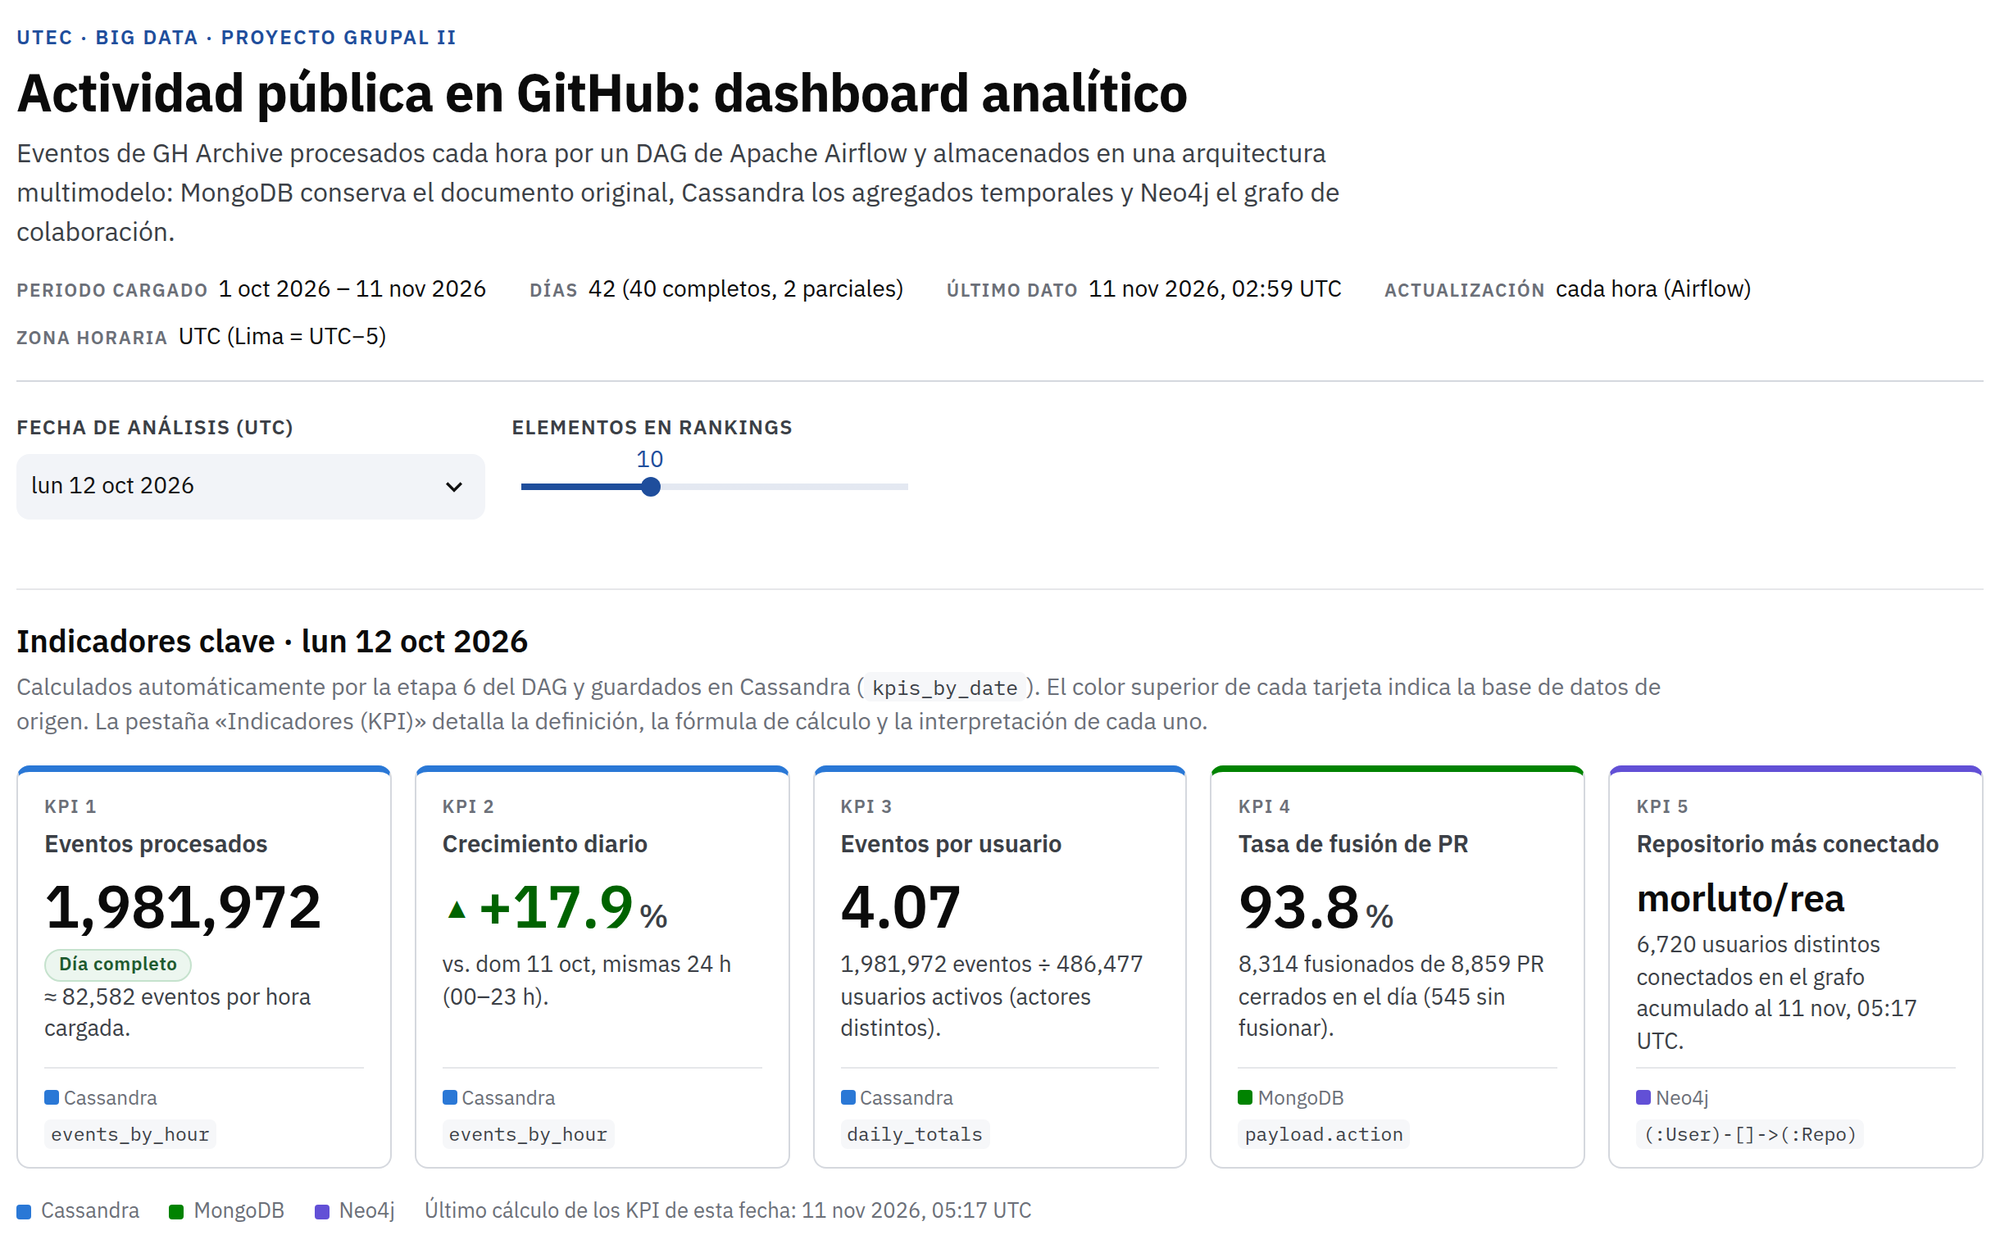
\includegraphics[width=\textwidth]{dash-encabezado.png}
    \caption{Encabezado del \textit{dashboard}: metadatos de cobertura, selector de fecha y tarjetas de los cinco KPI. El color del borde superior indica la base de datos de origen de cada indicador.}
    \label{fig:dash-encabezado}
\end{figure}

\begin{figure}[H]
    \centering
    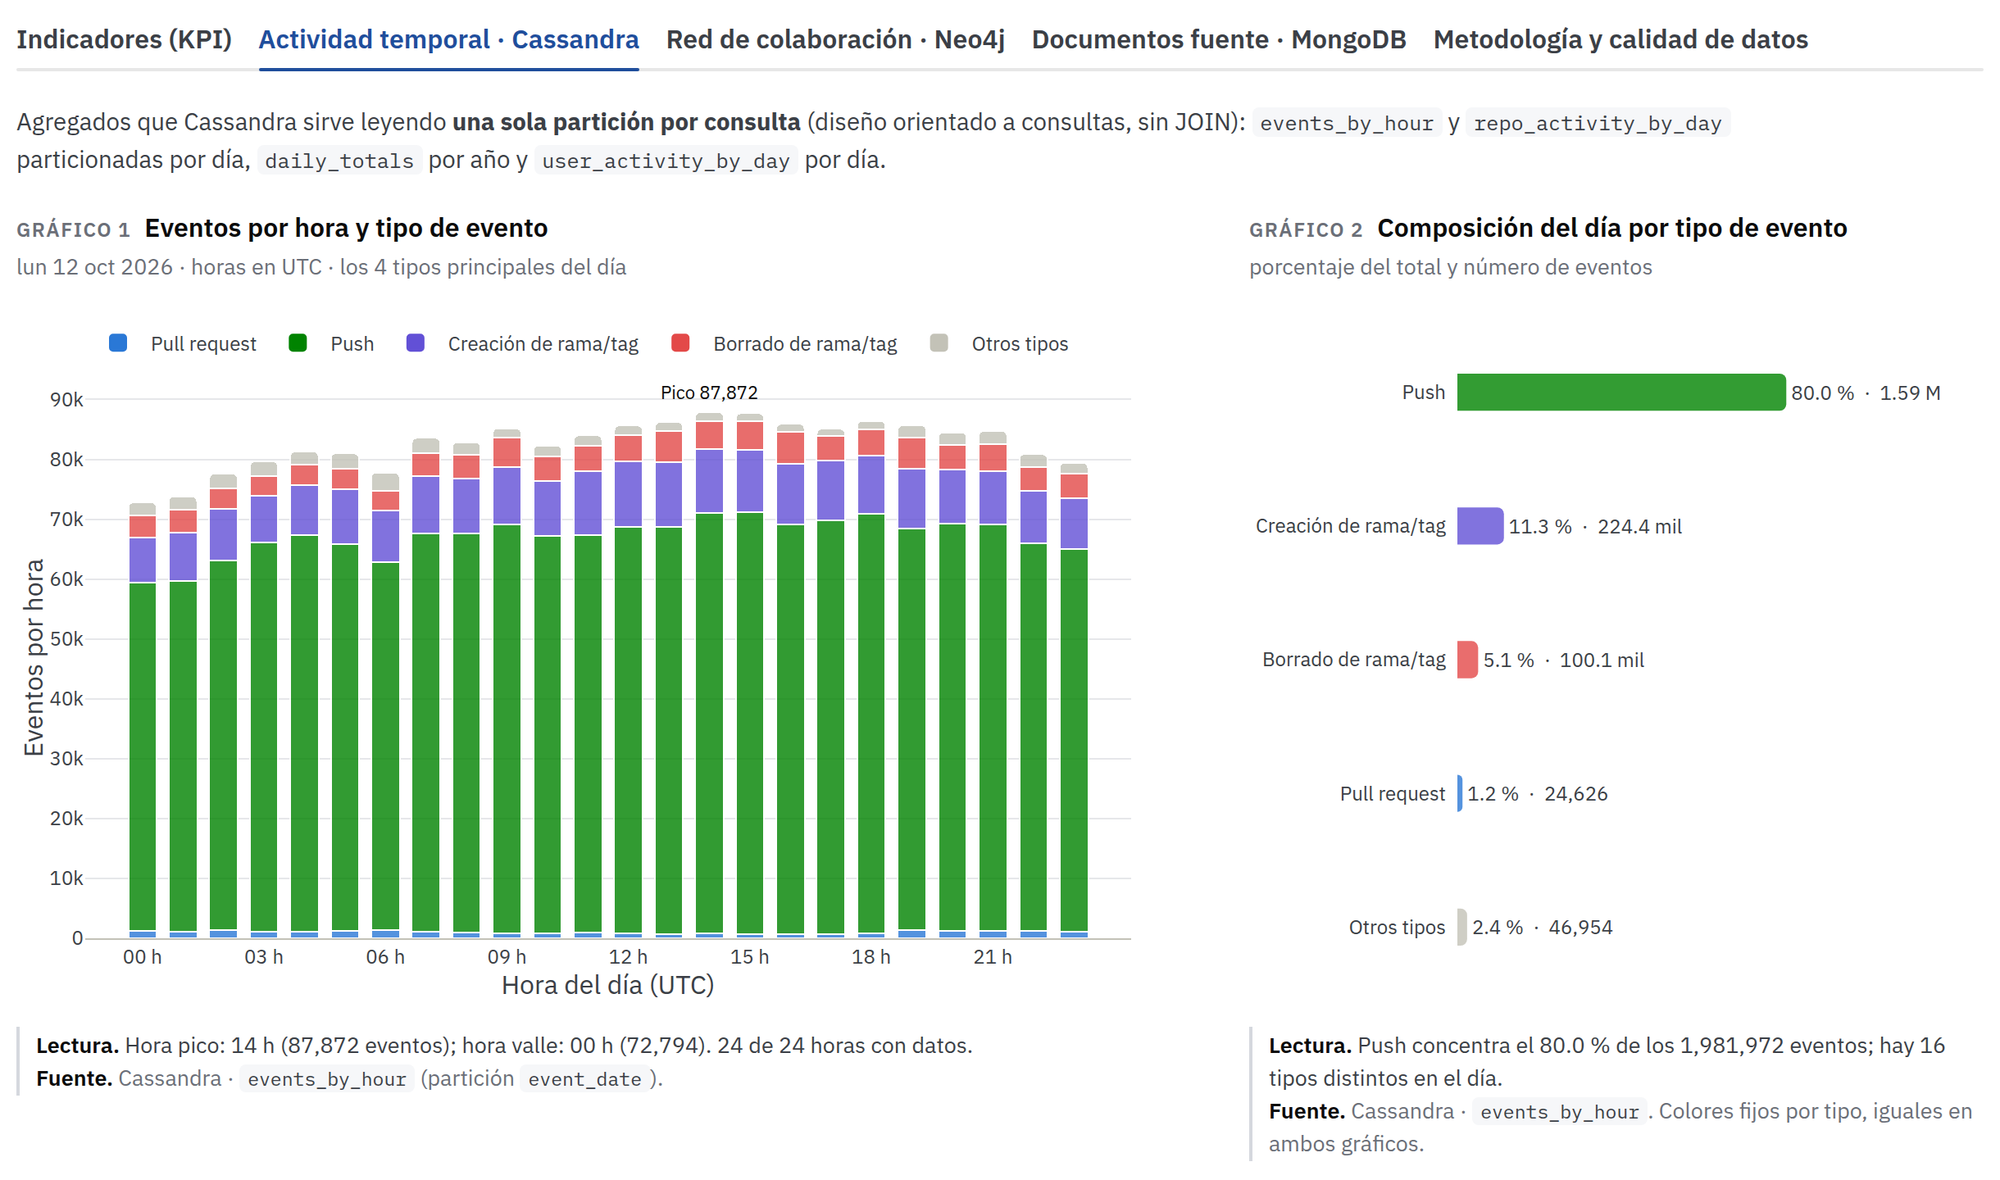
\includegraphics[width=\textwidth]{dash-cassandra-hora.png}
    \caption{Pestaña \guillemotleft{}Actividad temporal\guillemotright{} (Cassandra). Gráfico 1: eventos por hora y tipo. Gráfico 2: composición del día. Ambos se obtienen de una única partición de \texttt{events\_by\_hour}.}
    \label{fig:dash-cassandra-hora}
\end{figure}

\begin{figure}[H]
    \centering
    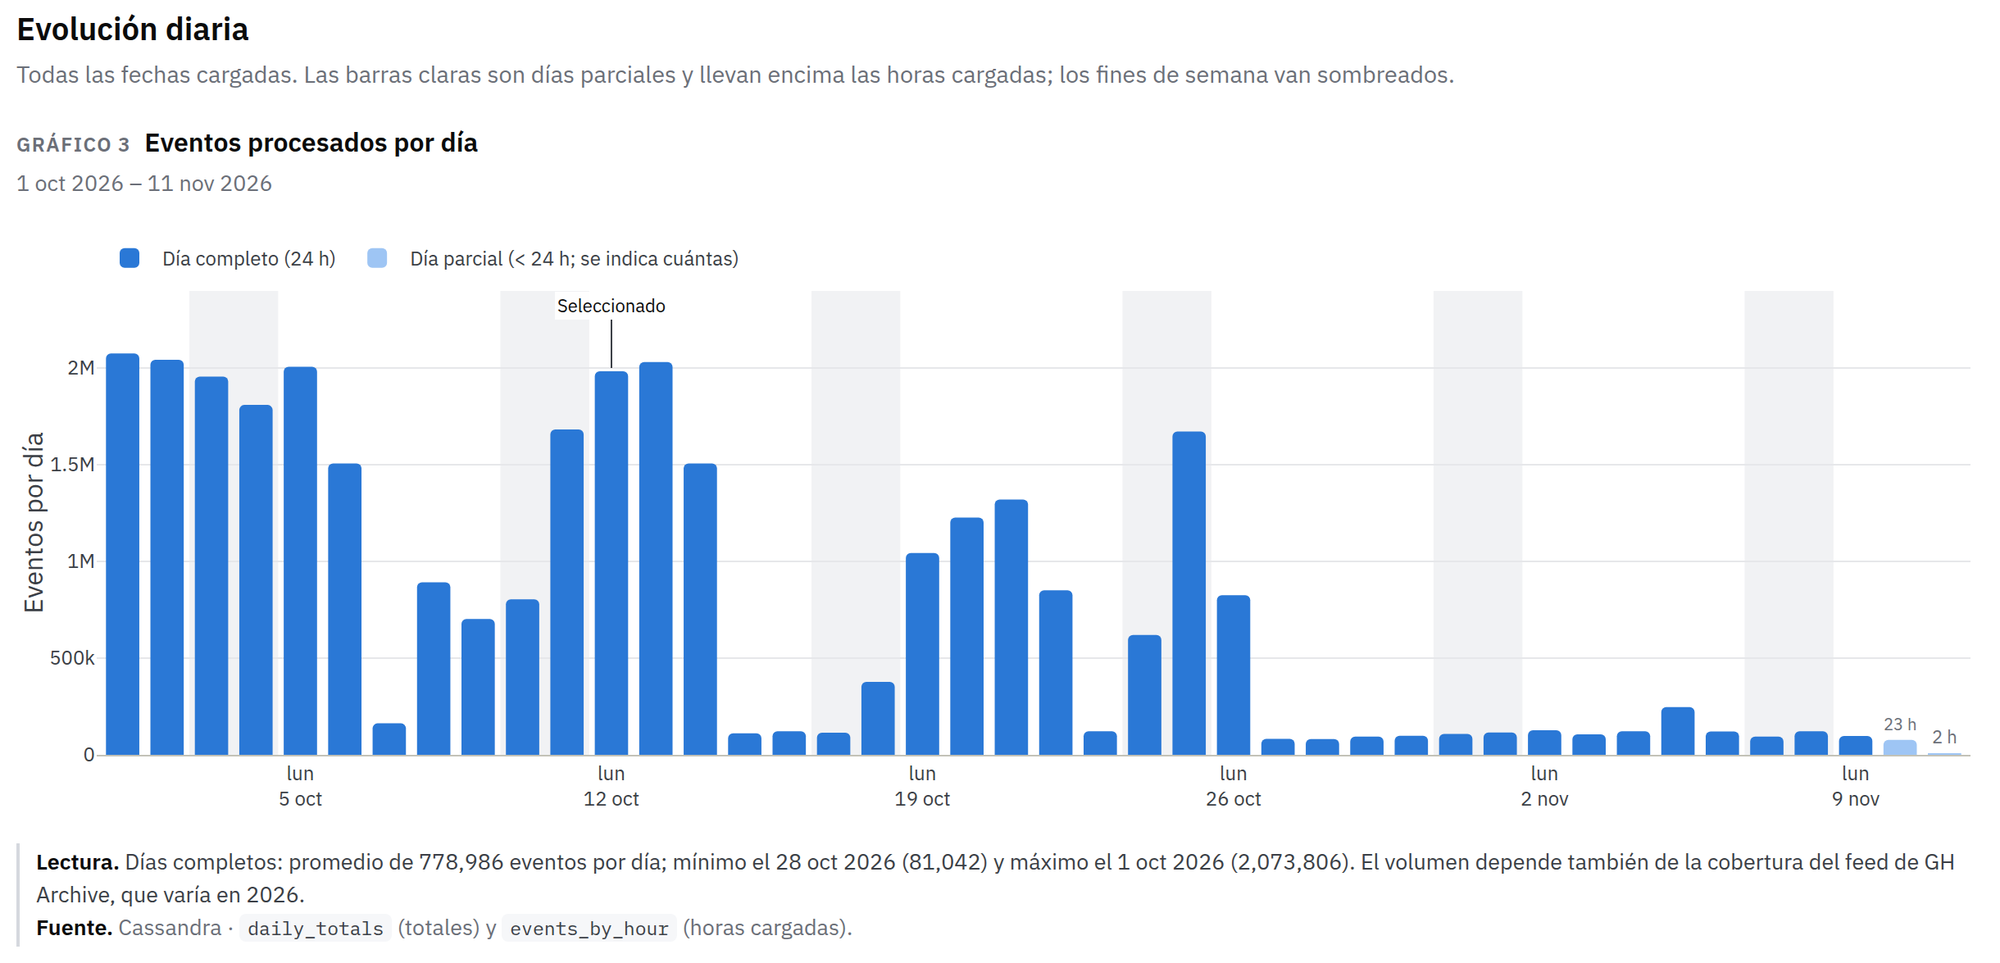
\includegraphics[width=\textwidth]{dash-cassandra-dia.png}
    \caption{Gráfico 3: eventos procesados por día en todo el periodo. Los escalones corresponden a la presencia o ausencia del flujo de referencias de Git en la fuente (Sección~\ref{subsec:cobertura}); las dos barras claras del extremo derecho son días parciales.}
    \label{fig:dash-cassandra-dia}
\end{figure}

\begin{figure}[H]
    \centering
    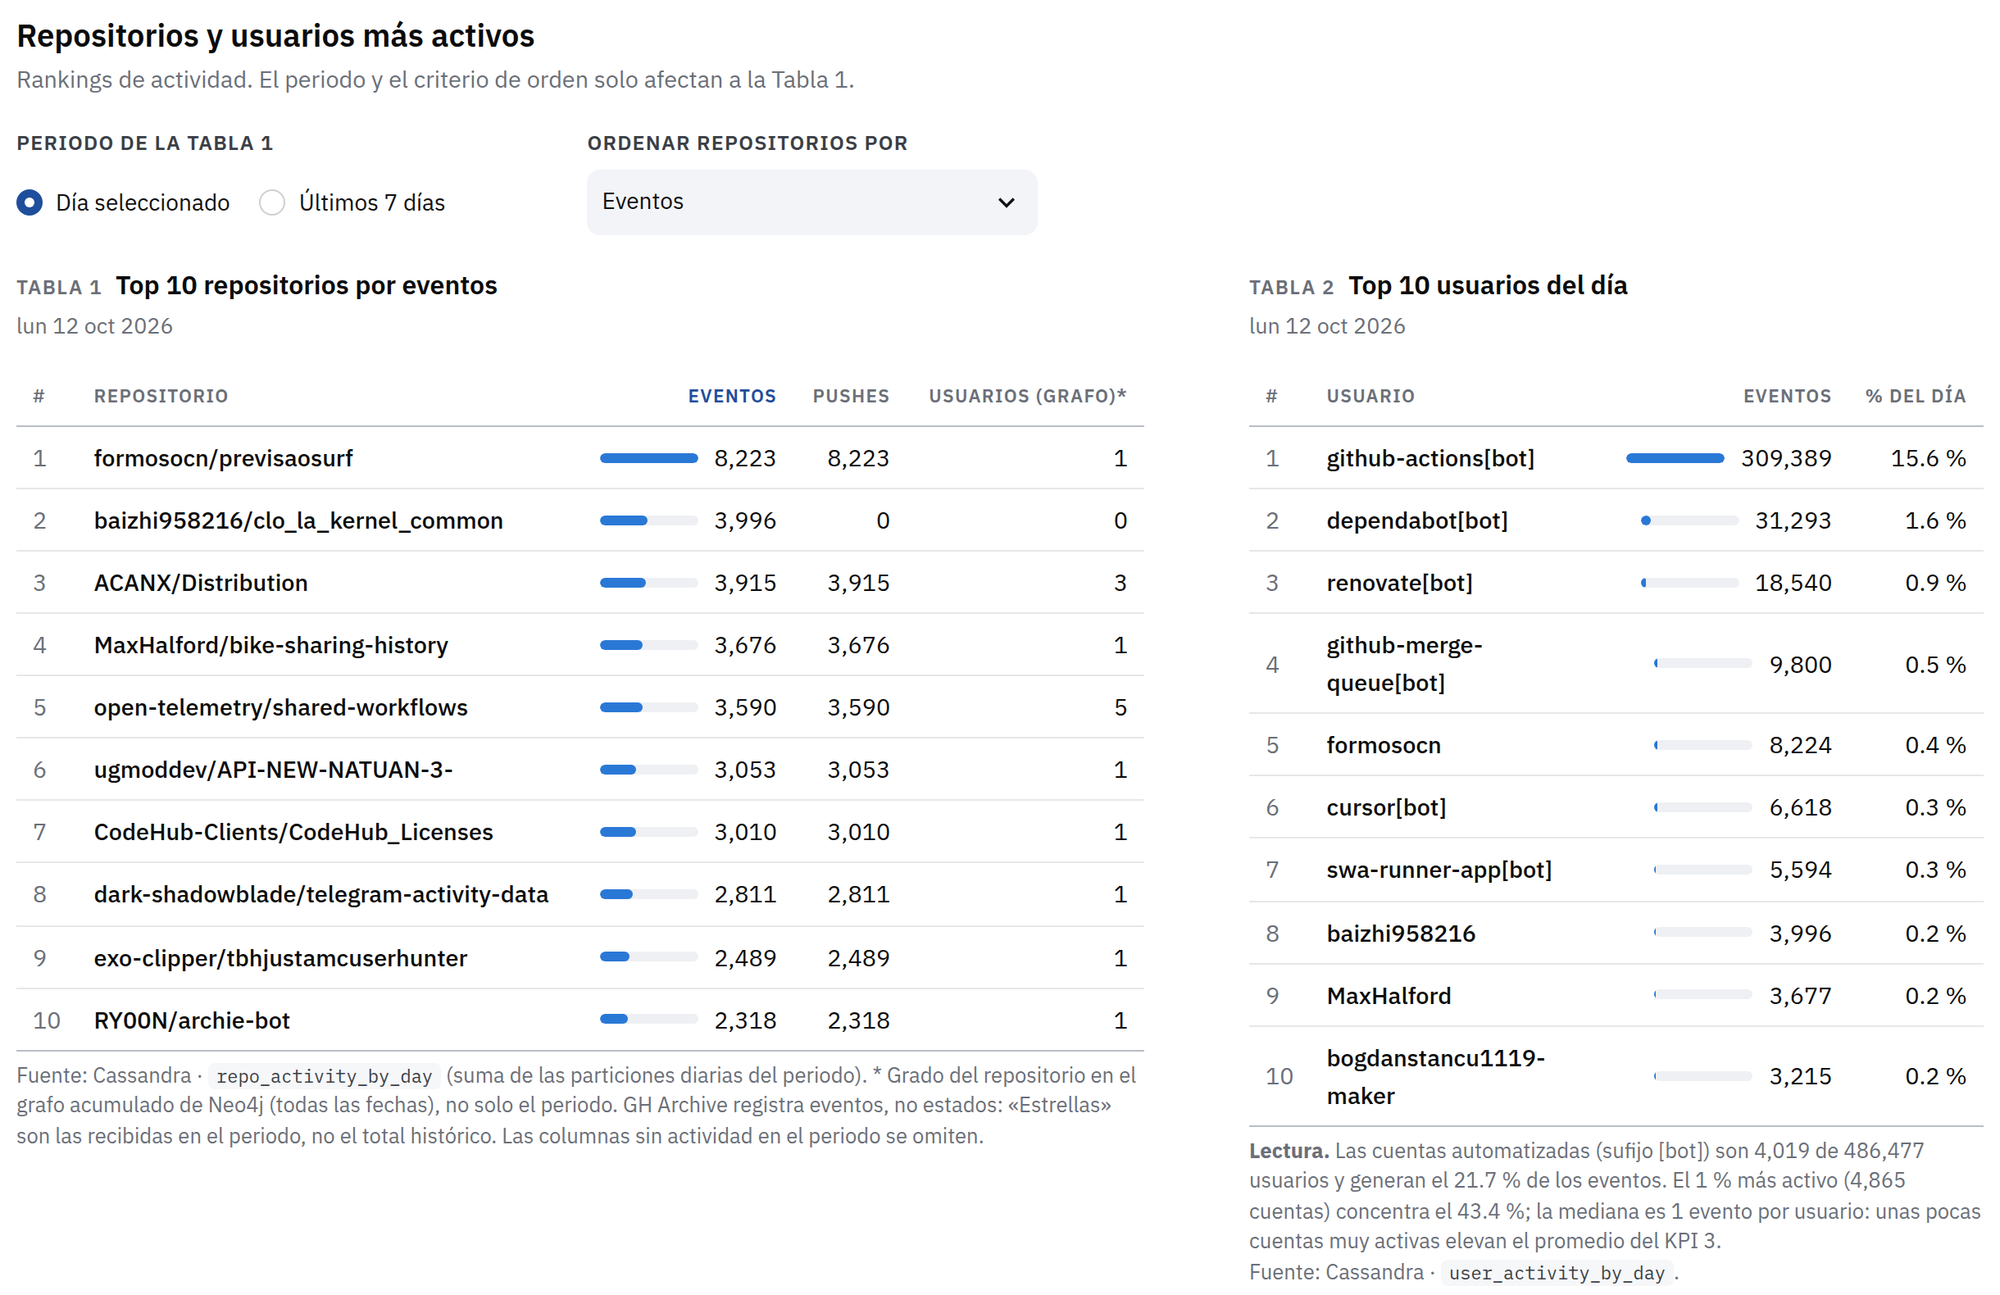
\includegraphics[width=\textwidth]{dash-cassandra-rankings.png}
    \caption{Tablas 1 y 2: repositorios y usuarios más activos del día. La columna \guillemotleft{}Usuarios (grafo)\guillemotright{} de la Tabla 1 cruza cada repositorio de Cassandra con su grado en Neo4j.}
    \label{fig:dash-cassandra-rankings}
\end{figure}

\begin{figure}[H]
    \centering
    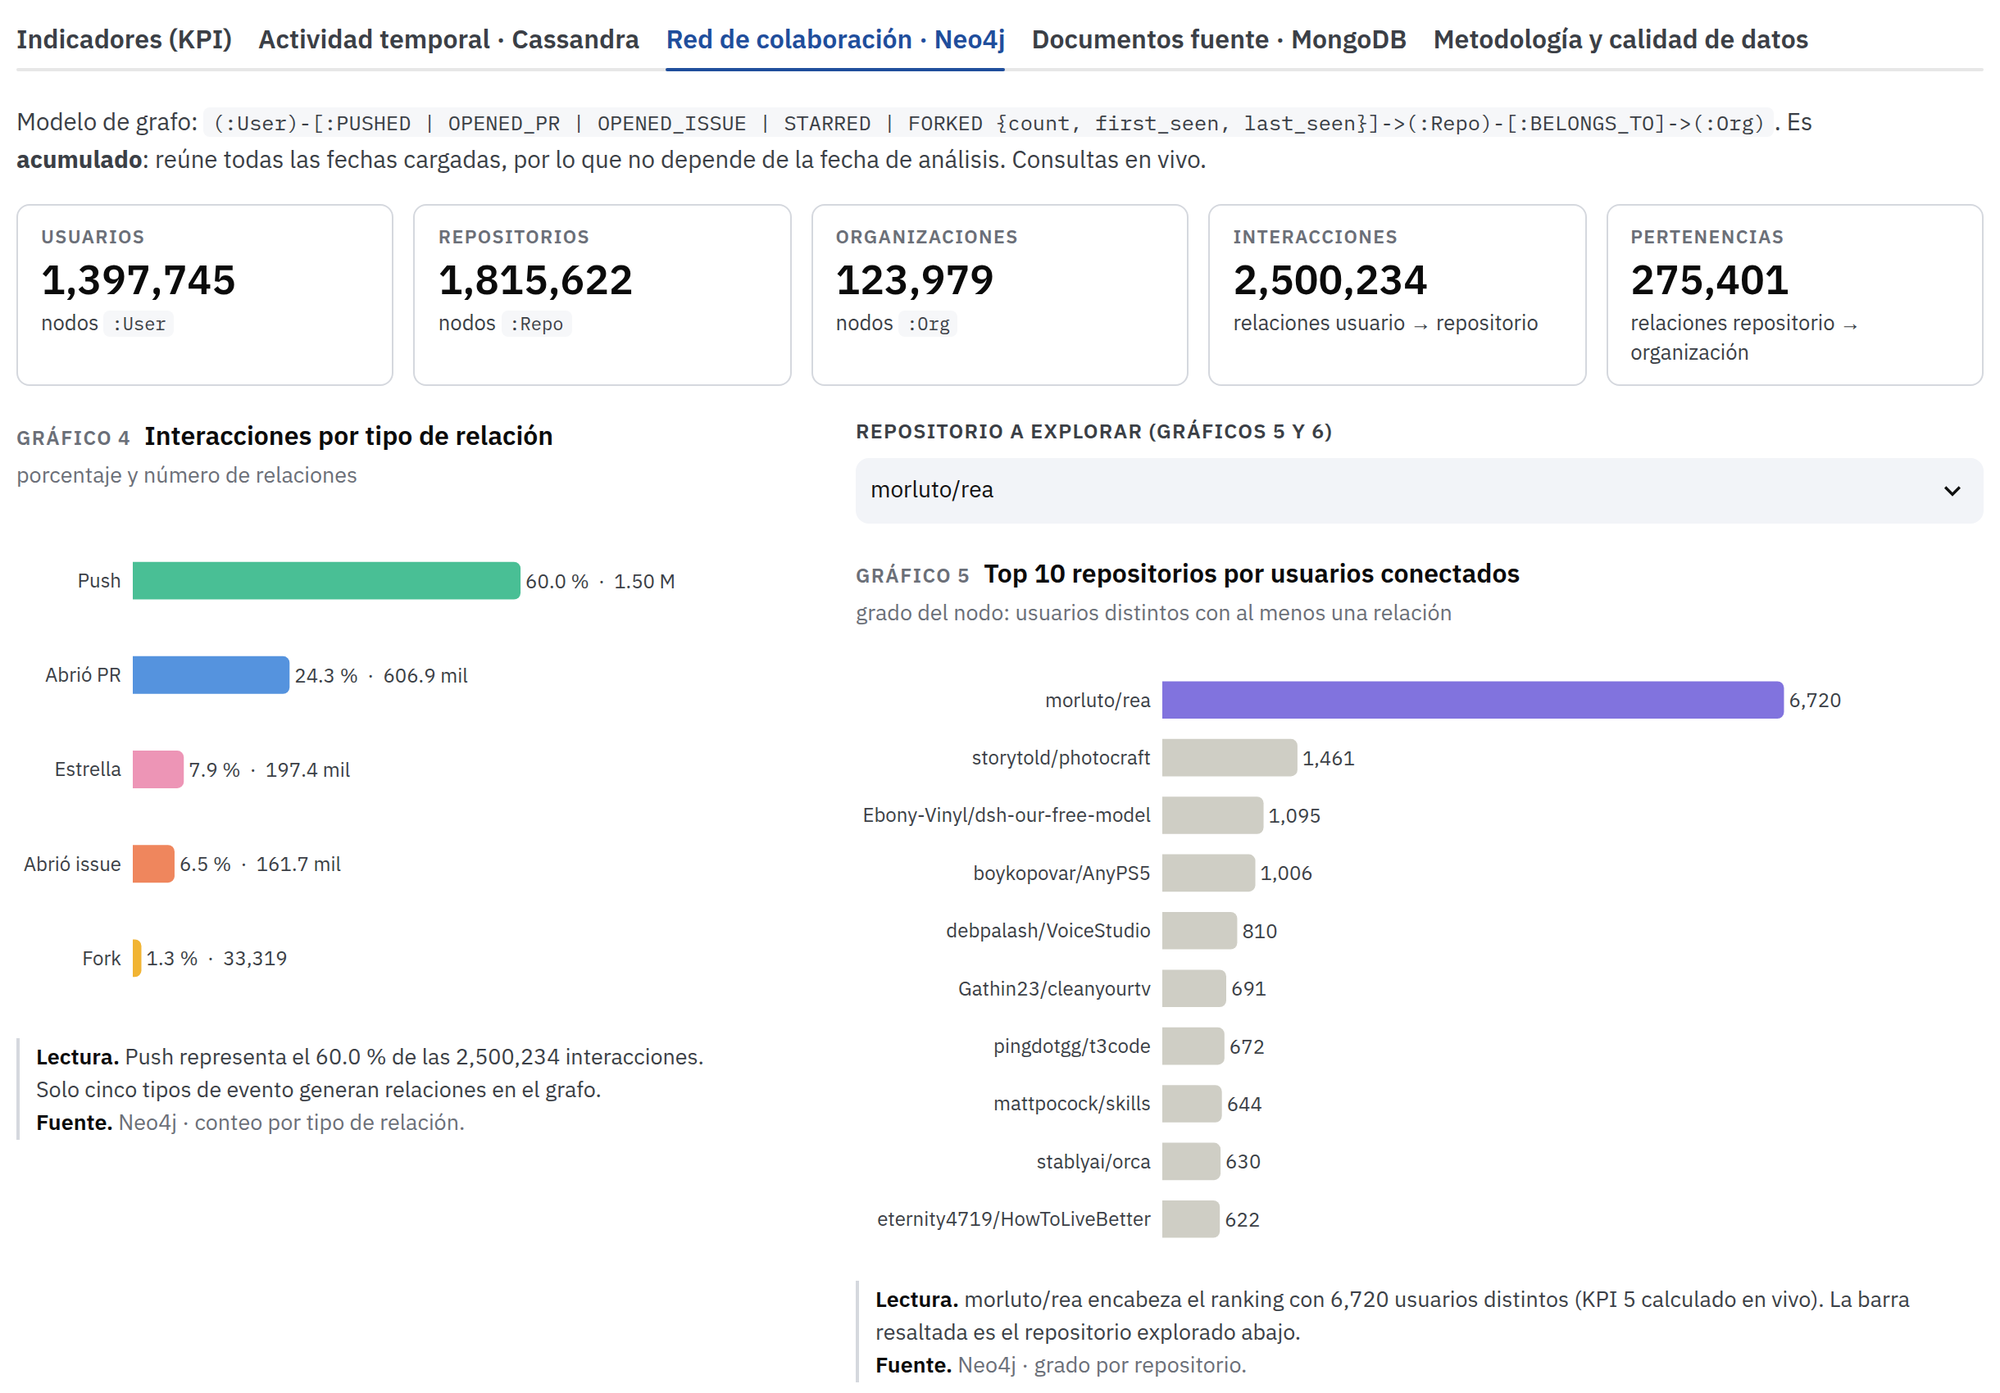
\includegraphics[width=\textwidth]{dash-neo4j-resumen.png}
    \caption{Pestaña \guillemotleft{}Red de colaboración\guillemotright{} (Neo4j). Tamaño del grafo, relaciones por tipo (Gráfico 4) y repositorios con más usuarios conectados (Gráfico 5).}
    \label{fig:dash-neo4j-resumen}
\end{figure}

\begin{figure}[H]
    \centering
    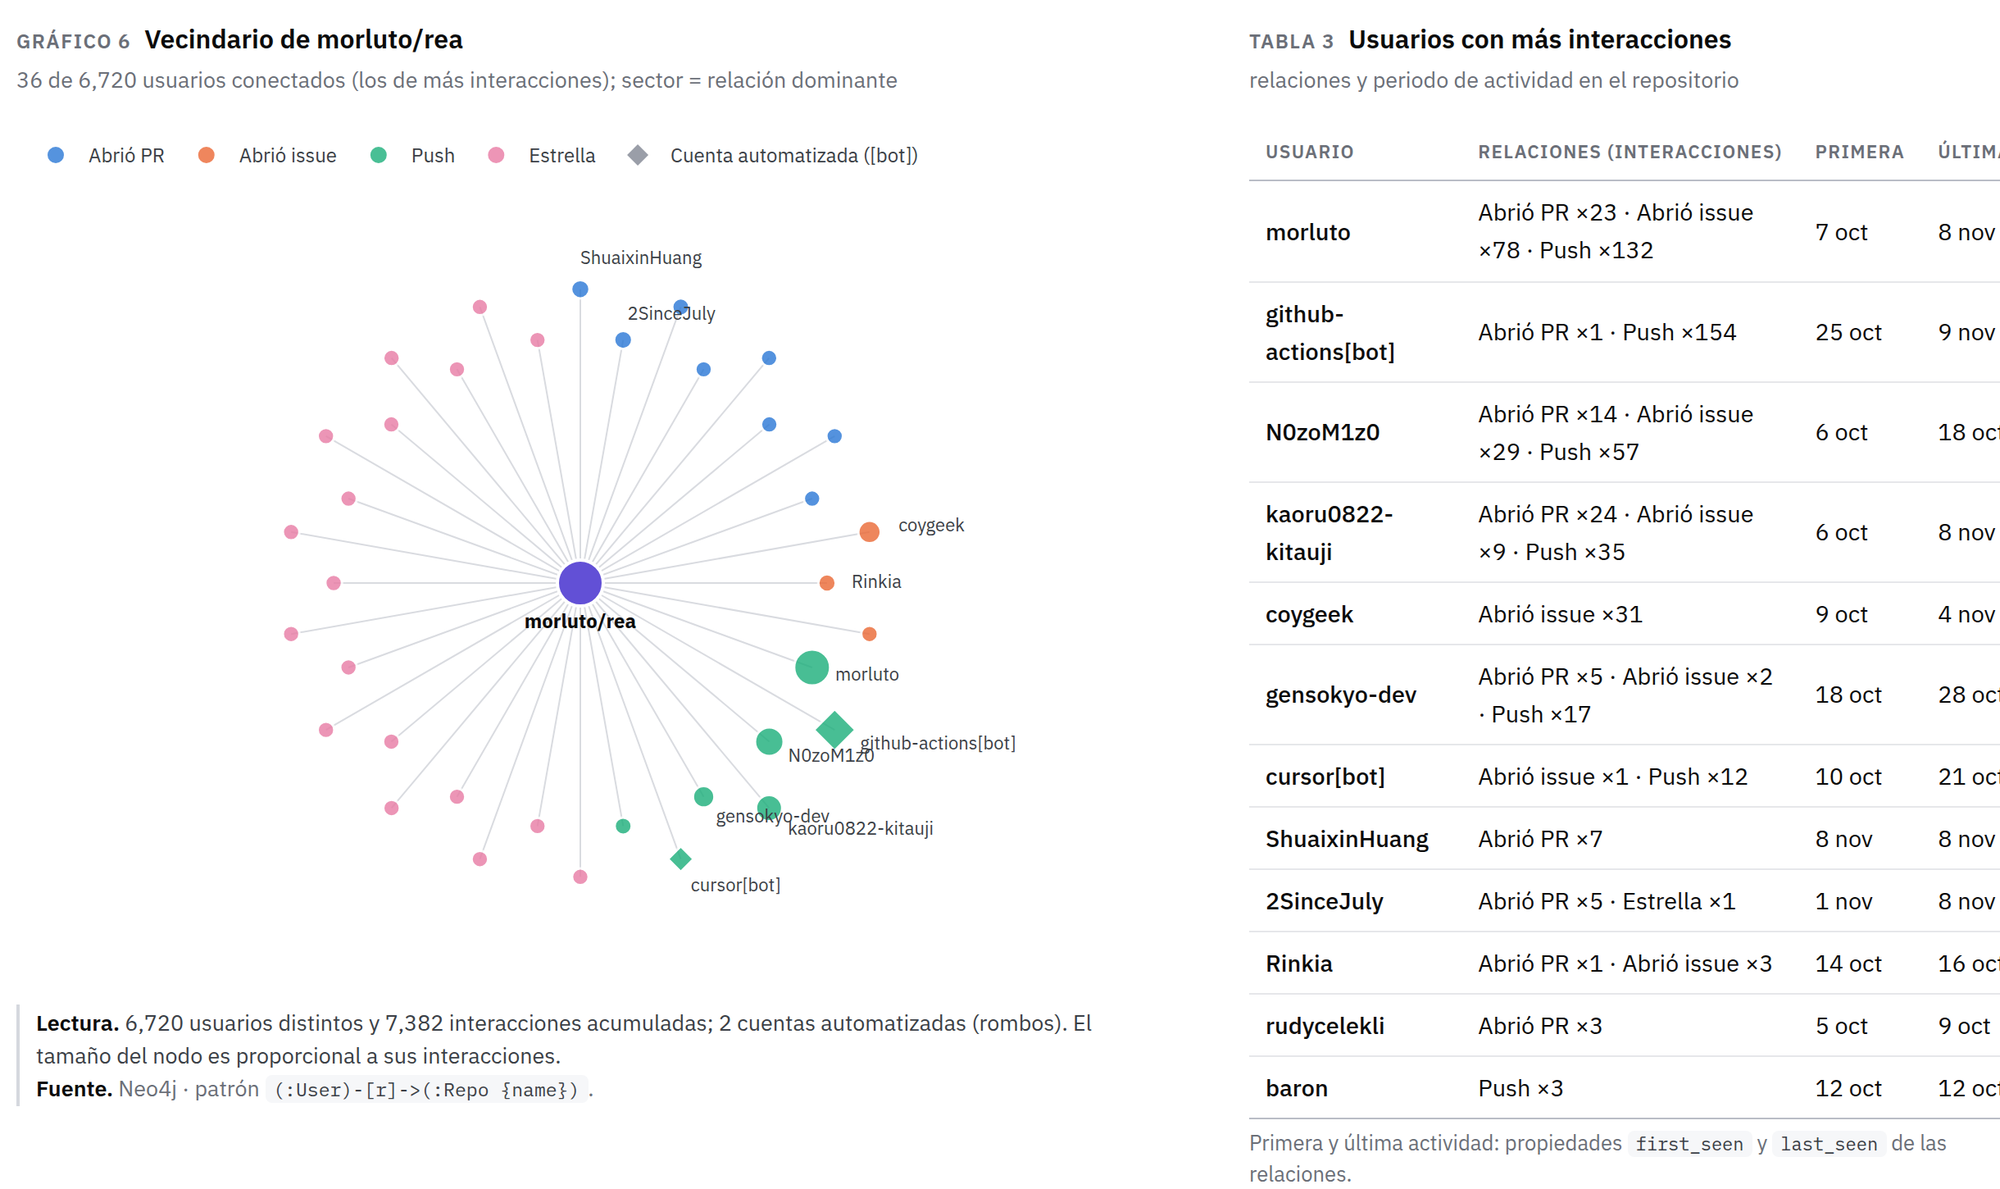
\includegraphics[width=\textwidth]{dash-neo4j-vecindario.png}
    \caption{Gráfico 6 y Tabla 3: vecindario del repositorio seleccionado. Se muestran los 36 usuarios con más interacciones; el color indica la relación dominante de cada uno y los rombos, cuentas automatizadas.}
    \label{fig:dash-neo4j-vecindario}
\end{figure}

\begin{figure}[H]
    \centering
    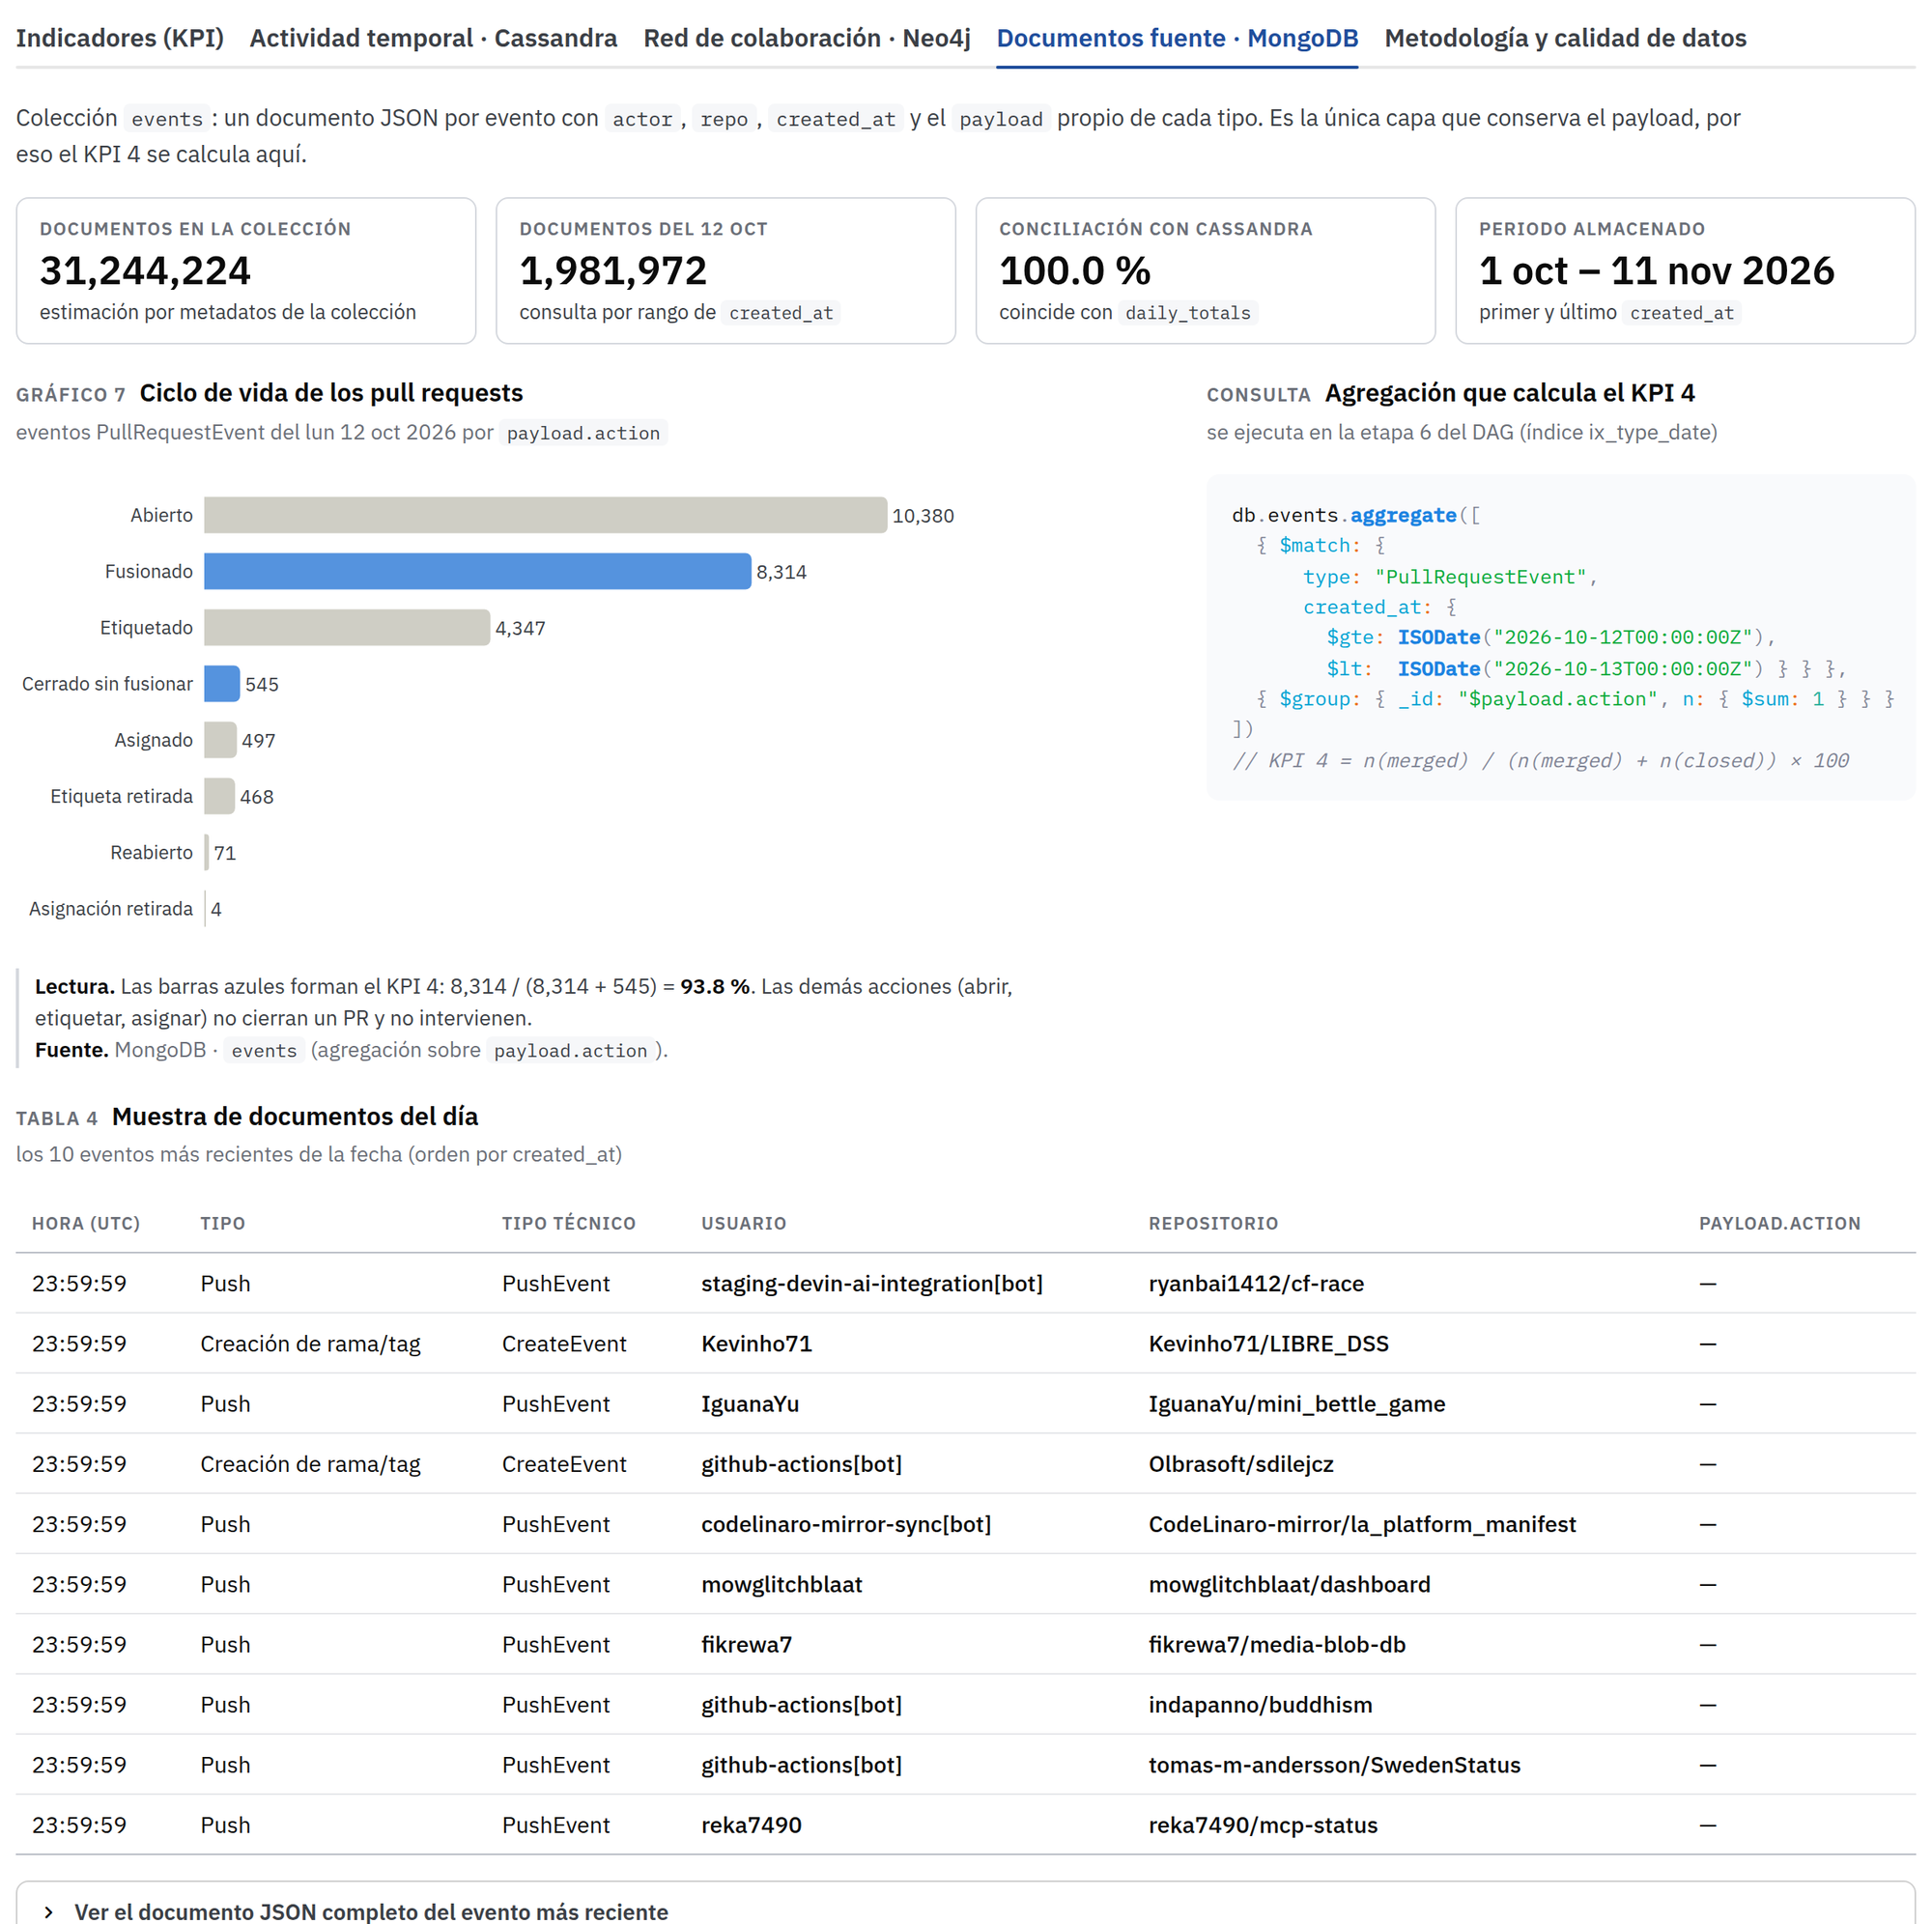
\includegraphics[width=0.96\textwidth]{dash-mongodb.png}
    \caption{Pestaña \guillemotleft{}Documentos fuente\guillemotright{} (MongoDB). La tarjeta de conciliación compara el conteo de documentos del día con el total de Cassandra (100\,\%). El Gráfico 7 muestra las acciones de los \textit{pull requests}; las dos barras resaltadas forman el KPI 4.}
    \label{fig:dash-mongodb}
\end{figure}

\begin{figure}[H]
    \centering
    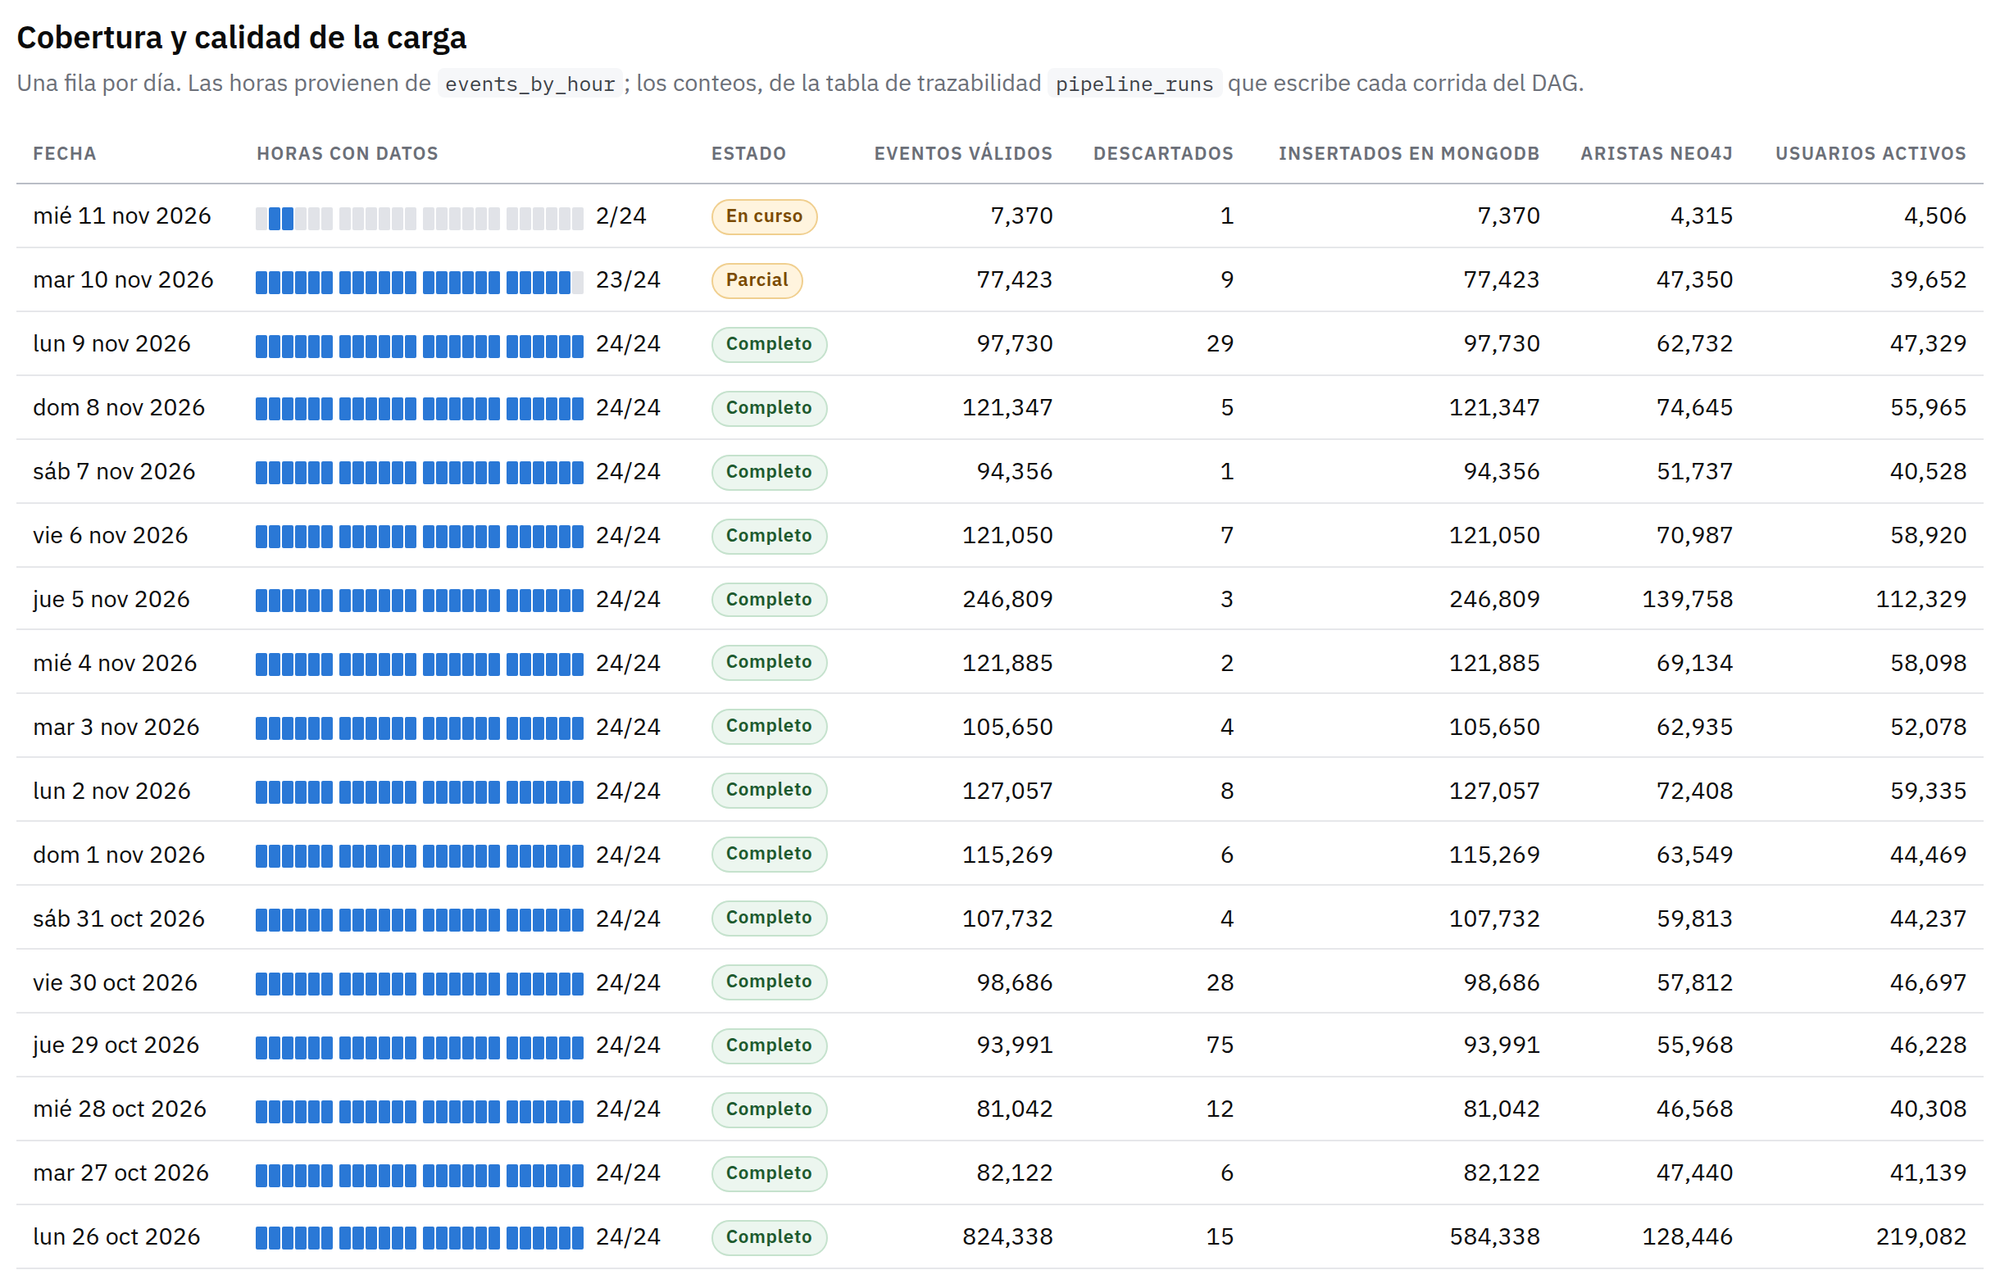
\includegraphics[width=\textwidth]{dash-cobertura.png}
    \caption{Pestaña \guillemotleft{}Metodología y calidad de datos\guillemotright{}: cobertura de la carga día por día (extracto), construida a partir de \texttt{events\_by\_hour} y de la tabla de trazabilidad \texttt{pipeline\_runs}.}
    \label{fig:dash-cobertura}
\end{figure}

\begin{figure}[H]
    \centering
    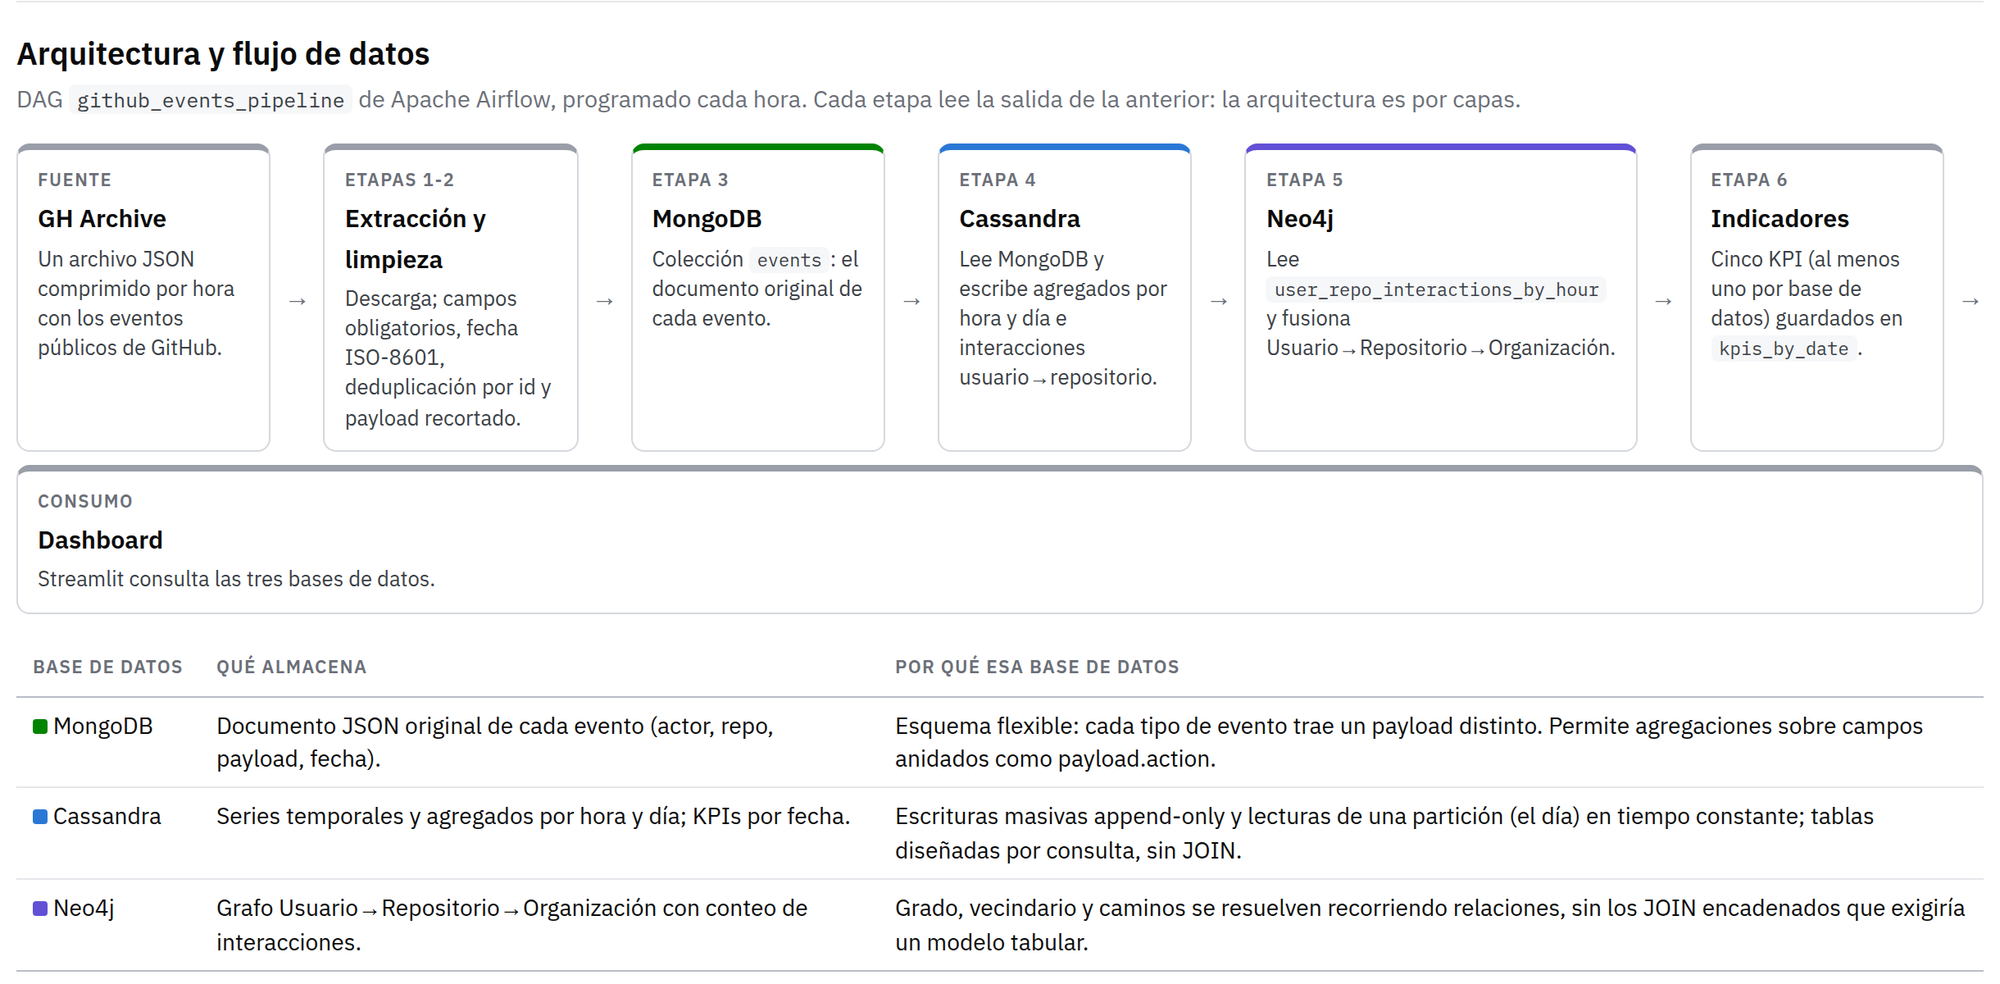
\includegraphics[width=\textwidth]{dash-arquitectura.png}
    \caption{El propio \textit{dashboard} documenta el flujo de datos y la justificación de cada base, de modo que quien lo consulta puede interpretar los indicadores sin recurrir a este informe.}
    \label{fig:dash-arquitectura}
\end{figure}
